\section{Experiments}
\label{sec:experiments}

\paragraph{Setup.} The encoder has 217M parameters (104M active per token) and the predictor 116M. The stems add 1.7M (linear) to 62M (convolutional) parameters over all product slots. We use AdamW~\cite{loshchilov2019decoupled} (weight decay 0.05, clipping at 1), bf16, linear warmup over 10\% of the steps and cosine decay, on 16--64 A100 GPUs with 96 to 3072 footprint rows per step and flash attention~\cite{dao2022flashattention} at $G{\geq}64$. Every 2.5k steps we validate on a fixed, seeded subset of the validation footprints with the block mask applied. All runs reported here use the single-observation configuration of \cref{sec:objective} ($K{=}1$, no state head, location embedding on all tokens, VICReg on evidence and predictions). Recipes changed as the project went on, so each comparison below changes one setting of one recipe (\cref{sec:supp_runs}), and all results are single runs. \TODO{multi-observation and state-head runs; see the planned experiments below}

\subsection{What pushes a run toward collapse}
\label{sec:ablations}

\begin{table}[t]
  \centering
  \footnotesize
  \setlength{\tabcolsep}{2.5pt}
  \caption{One-variable comparisons: $\Delta$ and $S$ at the same step in both arms. Background recipes differ between rows; the runs are listed in \cref{tab:supp_runs}. $^\dagger$The shared-canvas arm collapsed at this step and diverged shortly after; the fixed-GSD arm trained stably to 82.5k ($\Delta{=}0.060$, $S{=}0.38$).}
  \label{tab:ablations}
  \begin{tabular}{@{}lrcc@{}}
    \toprule
    Change (baseline $\to$ variant) & Step & $\Delta$ & $S$ \\
    \midrule
    Hinge on $\hat z$: $\gamma{=}1\to$ off        & 10k   & .010 $\to$ .055 & .77 $\to$ .24 \\
    Hinge on $\hat z$: $\gamma{=}1\to0.3$         & 2.5k  & .021 $\to$ .033 & .39 $\to$ .30 \\
    Covariance $w_c$: $0.005\to0.05$              & 8k    & .204 $\to$ .003 & .38 $\to$ .90 \\
    4 MoE layers $\to$ dense                      & 97.5k & .167 $\to$ .094 & .16 $\to$ .52 \\
    Kernel floor $k_{\min}$: $1\to4$              & 97.5k & .167 $\to$ .121 & .16 $\to$ .25 \\
    Shared canvas $\to$ fixed-GSD$^\dagger$       & 65k   & .127 $\to$ .045 & .67 $\to$ .56 \\
    Grid $G$: $64\to32$                           & 10k   & .010 $\to$ .009 & .77 $\to$ .55 \\
    Grid $G$: $64\to128$                          & 10k   & .010 $\to$ .016 & .77 $\to$ .63 \\
    \bottomrule
  \end{tabular}
\end{table}

\begin{figure*}[t]
  \centering
  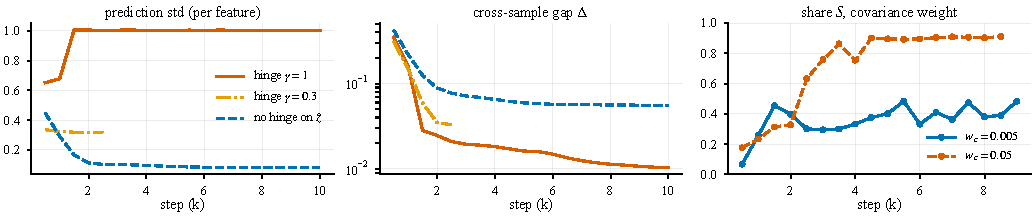
\includegraphics[width=\textwidth]{figures/regularizers.pdf}
  \caption{Two regularizers that pull the wrong way. \emph{Left, middle:} with the variance hinge on the predictions ($\gamma{=}1$), their per-feature standard deviation jumps to 1 at 1.5k steps and $\Delta$ drops fivefold within 500 steps. Without it, the standard deviation settles near 0.08 and $\Delta$ ends 5.3 times higher. The $\gamma{=}0.3$ run stopped early. \emph{Right:} a covariance weight of 0.05 sends a standard-attention model into a position code by 4k steps.}
  \label{fig:regularizers}
\end{figure*}

\paragraph{The variance hinge fights calibration.} The VICReg variance term asks for a per-feature standard deviation of at least $\gamma$ across tokens. That sounds harmless for layer-normalized targets, but a calibrated prediction $\E[\bar z\mid\text{source}]$ has a standard deviation of about $\sqrt{R^2}$, where $R^2$ is the share of the target's variance the source explains. Ours is around 1\%, so the hinge asks for ten times the calibrated spread. The cheapest variance to add without raising the loss is structure that the target also has and the predictor can produce without reading the source: $u$, $m_t$ and $l$ of \cref{eq:decomp}. With the hinge, the prediction standard deviation snaps to 1 and $\Delta$ drops fivefold within 500 steps (\cref{fig:regularizers}). Turning it off for the predictions (it stays on the evidence) gives 5.3 times the gap at 10k steps, $S$ of 0.24 instead of 0.77 and a lower validation loss (0.350 vs.\ 0.390), and $\gamma{=}0.3$ falls in between. The hinge is on in every other run in this paper, including the downstream backbone, and probably explains part of their early trough. In the recipe of \cref{sec:objective} the hinge acts only on the state head.

\paragraph{Covariance and experts.} Raising $w_c$ from 0.005 to 0.05 turned a standard-attention model into a position code within 4k steps, as \cref{sec:blind} predicts. Removing the four MoE layers lowered the late gap from 0.167 to 0.094 and raised $S$ from 0.16 to 0.52, while the validation loss improved (0.168 vs.\ 0.189). The routers were not trouble-free: in three long runs the first MoE layer lost balance before the gradient norm grew, and one run ended with three quarters of its experts unused.

\subsection{Tokenization}
\label{sec:exp_tokens}

\paragraph{Fixed-GSD stems vs.\ a shared canvas.} With five products and nothing else changed, the shared-canvas model reached the higher gap (0.169 at 55k steps) but then collapsed dimensionally (rank 623 $\to$ 402) and diverged at 66k. The fixed-GSD model held its rank near 610 and trained stably to the end of its allocation at 82.5k. The two stems produce different targets, so their gap values are not comparable; their stability is.

\paragraph{Kernel floor.} The floor does what it was meant to do (\cref{tab:floor}). With $k_{\min}{=}1$, pairs involving LOLA roughness were close to chance ($\Delta{=}0.033$ as target, 0.023 as source). With $k_{\min}{=}4$ they rose three- to fourfold, and TiO$_2$ gained as a target. The other pairs lost ground (0.205 $\to$ 0.122), and so did the overall gap. With one seed per arm we cannot tell a trade-off from run-to-run variation.

\paragraph{Grid size.} In a 10k-step sweep that changed only $G$, the validation loss improved with resolution (0.420, 0.390, 0.364 for $G{=}32, 64, 128$), and $G{=}128$ ended with the largest training-window gap on 11 of 12 target products. On 32 GPUs the runs took 24, 28 and 63 hours. All three had the variance hinge on and ended in the trough of \cref{sec:monitor}, so the numbers rank the grids but understate them. We use $G{=}64$ as the compromise.

\paragraph{Dense-prediction upgrades.} The dense context loss (\cref{eq:ctx}) and the convolutional stems both aim at better features per cell. Trained together at $G{=}32$ with shared-canvas stems and seven products, they raised $\Delta$ from 0.19 at the first validation (2.5k steps) to 0.308 at 10k instead of dropping into the trough, and held 0.294 at 35k, with $S$ between 0.05 and 0.23. The closest earlier run shares grid, products, learning rate, batch and regularizers and reached $\Delta{=}0.064$ ($S{=}0.45$) at 35k; it differs in normalization statistics, validation subset and code version, so the comparison is confounded. \TODO{clean ablation with both upgrades off, and the $G{=}64$ runs on both stem types}

\subsection{Downstream}
\label{sec:downstream}

The downstream results use an earlier checkpoint ($G{=}64$, shared-canvas stems, six products, 79k steps at a peak learning rate of $10^{-4}$, variance hinge on). Its transformer is always frozen. The crater detectors fine-tune the per-product stems with their heads, and the probes read frozen features only (\cref{sec:supp_downstream}).

\begin{table}[t]
  \centering
  \footnotesize
  \setlength{\tabcolsep}{3.5pt}
  \caption{Crater detection with a frozen encoder and fine-tuned stems (test split, single seed). \emph{Top:} FCOS heads~\cite{tian2019fcos} with our neck. \emph{Bottom:} the NASA-IBM LFM protocol (Faster R-CNN family, WAC only, boxes of at least 10\,px, at most 500 detections).}
  \label{tab:craters}
  \begin{tabular}{@{}llcc@{}}
    \toprule
    Data & Input & mAP$_{50}$ & mAP \\
    \midrule
    Robbins, 1k tiles  & WAC                     & 0.530 & 0.238 \\
                       & WAC + predicted DTM     & 0.549 & 0.242 \\
                       & WAC + DTM               & 0.595 & 0.285 \\
    Robbins, 10k tiles & WAC                     & 0.530 & 0.270 \\
                       & WAC + DTM               & \textbf{0.755} & \textbf{0.411} \\
    NAC, hand-labeled  & NAC                     & 0.690 & 0.319 \\
    \midrule
    \multicolumn{2}{@{}l}{NASA-IBM LFM~\cite{fraccaro2026multimodal}, our reproduction} & 0.464 & 0.190 \\
    \multicolumn{2}{@{}l}{Ours, LFM detection stack}                  & 0.362 & 0.156 \\
    \multicolumn{2}{@{}l}{Ours, our neck + jitter, tokens only}       & 0.433 & 0.187 \\
    \multicolumn{2}{@{}l}{Ours, our neck + jitter + pixel branch}     & \textbf{0.494} & \textbf{0.217} \\
    \bottomrule
  \end{tabular}
\end{table}

\paragraph{Crater detection.} We train detection heads for the Robbins catalog~\cite{robbins2019new} on WAC tiles at 100\,m (1k and 10k tiles) and for hand-labeled NAC craters at 0.8--5\,m from six of the ten NAC photometry sites of SomBench~\cite{patil2026sombench} (\cref{tab:craters}). Adding the DTM as a second input to the same frozen backbone is the largest single effect: $+0.065$ mAP$_{50}$ with 1k tiles and $+0.225$ with 10k tiles, where the lighting varies more. A DTM that the backbone itself predicts from the WAC image recovers 0.019 of the 0.065. For a comparison with the NASA-IBM lunar foundation model~\cite{fraccaro2026multimodal}, which is trained by masked token prediction, we reproduced its frozen-backbone Faster R-CNN protocol on the same data and obtained 0.464 mAP$_{50}$ for that model, against 0.458 reported. With its detection stack our tokens reach 0.362--0.390. With our neck and scale jitter they reach 0.433 from tokens alone, and 0.494 when the detector also gets a raw-pixel branch. Our fine-tuned stems favor us in this comparison, so we read it as rough parity on single-product craters. The distinctive gain comes from the second product.

\paragraph{Shape, albedo and shadows.} A WAC image mixes topography, albedo and illumination, and the backbone was never trained to separate them. We probe whether its predictions do, on 40 held-out footprints seen under eight suns each (all metrics in \cref{tab:safs}). Given only a WAC image, linear probes on the predictor features for the elevation and 643\,nm products recover relief with correlation 0.705 (0.12 for the same probe on pixels) and albedo with 0.840. Both barely change with the sun, and the predicted relief picks the right footprint among the 40 in 96\% of cases. A small head that integrates the backbone's own slope and aspect predictions reaches a relief RMSE of 299\,m (551\,m for zero relief). The reverse direction tests the sun conditioning. From topography and a sun, a linear probe on the predictor's WAC features localizes cast shadows with AUC 0.89, against 0.59 with another observation's sun and 0.49 with none. The predictor uses the sun it is given.

\subsection{Planned experiments}
\label{sec:planned}

The recipe of \cref{sec:method} is being trained on the corpus of \cref{sec:dataset}; the comparisons below are designed, and their tables will replace the TODOs. \emph{(E1) Observations and state.} At matched budget, $K{=}1$ without the state head (the configuration above) against $K\in\{1,2,3\}$ with it, scored by $\Delta$, by the content and position probes of \cref{sec:supp_runs}, and by the downstream tasks. \emph{(E2) Relighting.} The repeat-acquisition task on and off, scored by the sun-swap shadow test and by how much the state $\hat w$ of one footprint changes between its observations. \emph{(E3) Location.} The location embedding on all tokens, on the predictor only with dropout, and absent, to measure how much of $\Delta$ the $l$ term of \cref{eq:decomp} accounts for. \emph{(E4) Monitors.} Over all checkpoints, each monitor as a detector of the probe labels, with AUROC and lead time. \emph{(E5) Baselines.} The NASA-IBM model~\cite{fraccaro2026multimodal}, DINOv3~\cite{simeoni2026dinov3} and a random encoder on crater detection, irregular mare patch segmentation~\cite{braden2014evidence,patil2026sombench} and polar ice prospectivity, with LunarFM~\cite{gironamata2026lunarfm} and Moonstone~\cite{prasad2026moonstone} where weights are available.
